\chapter{Materials and Devices}
In this chapter, the redox conductive polymers are presented and a preparation of organic electrochemical half-cells suitable for electron spin resonance spectroscopy is described.

\section{Electrolytes}
\begin{figure}[h]
\center
	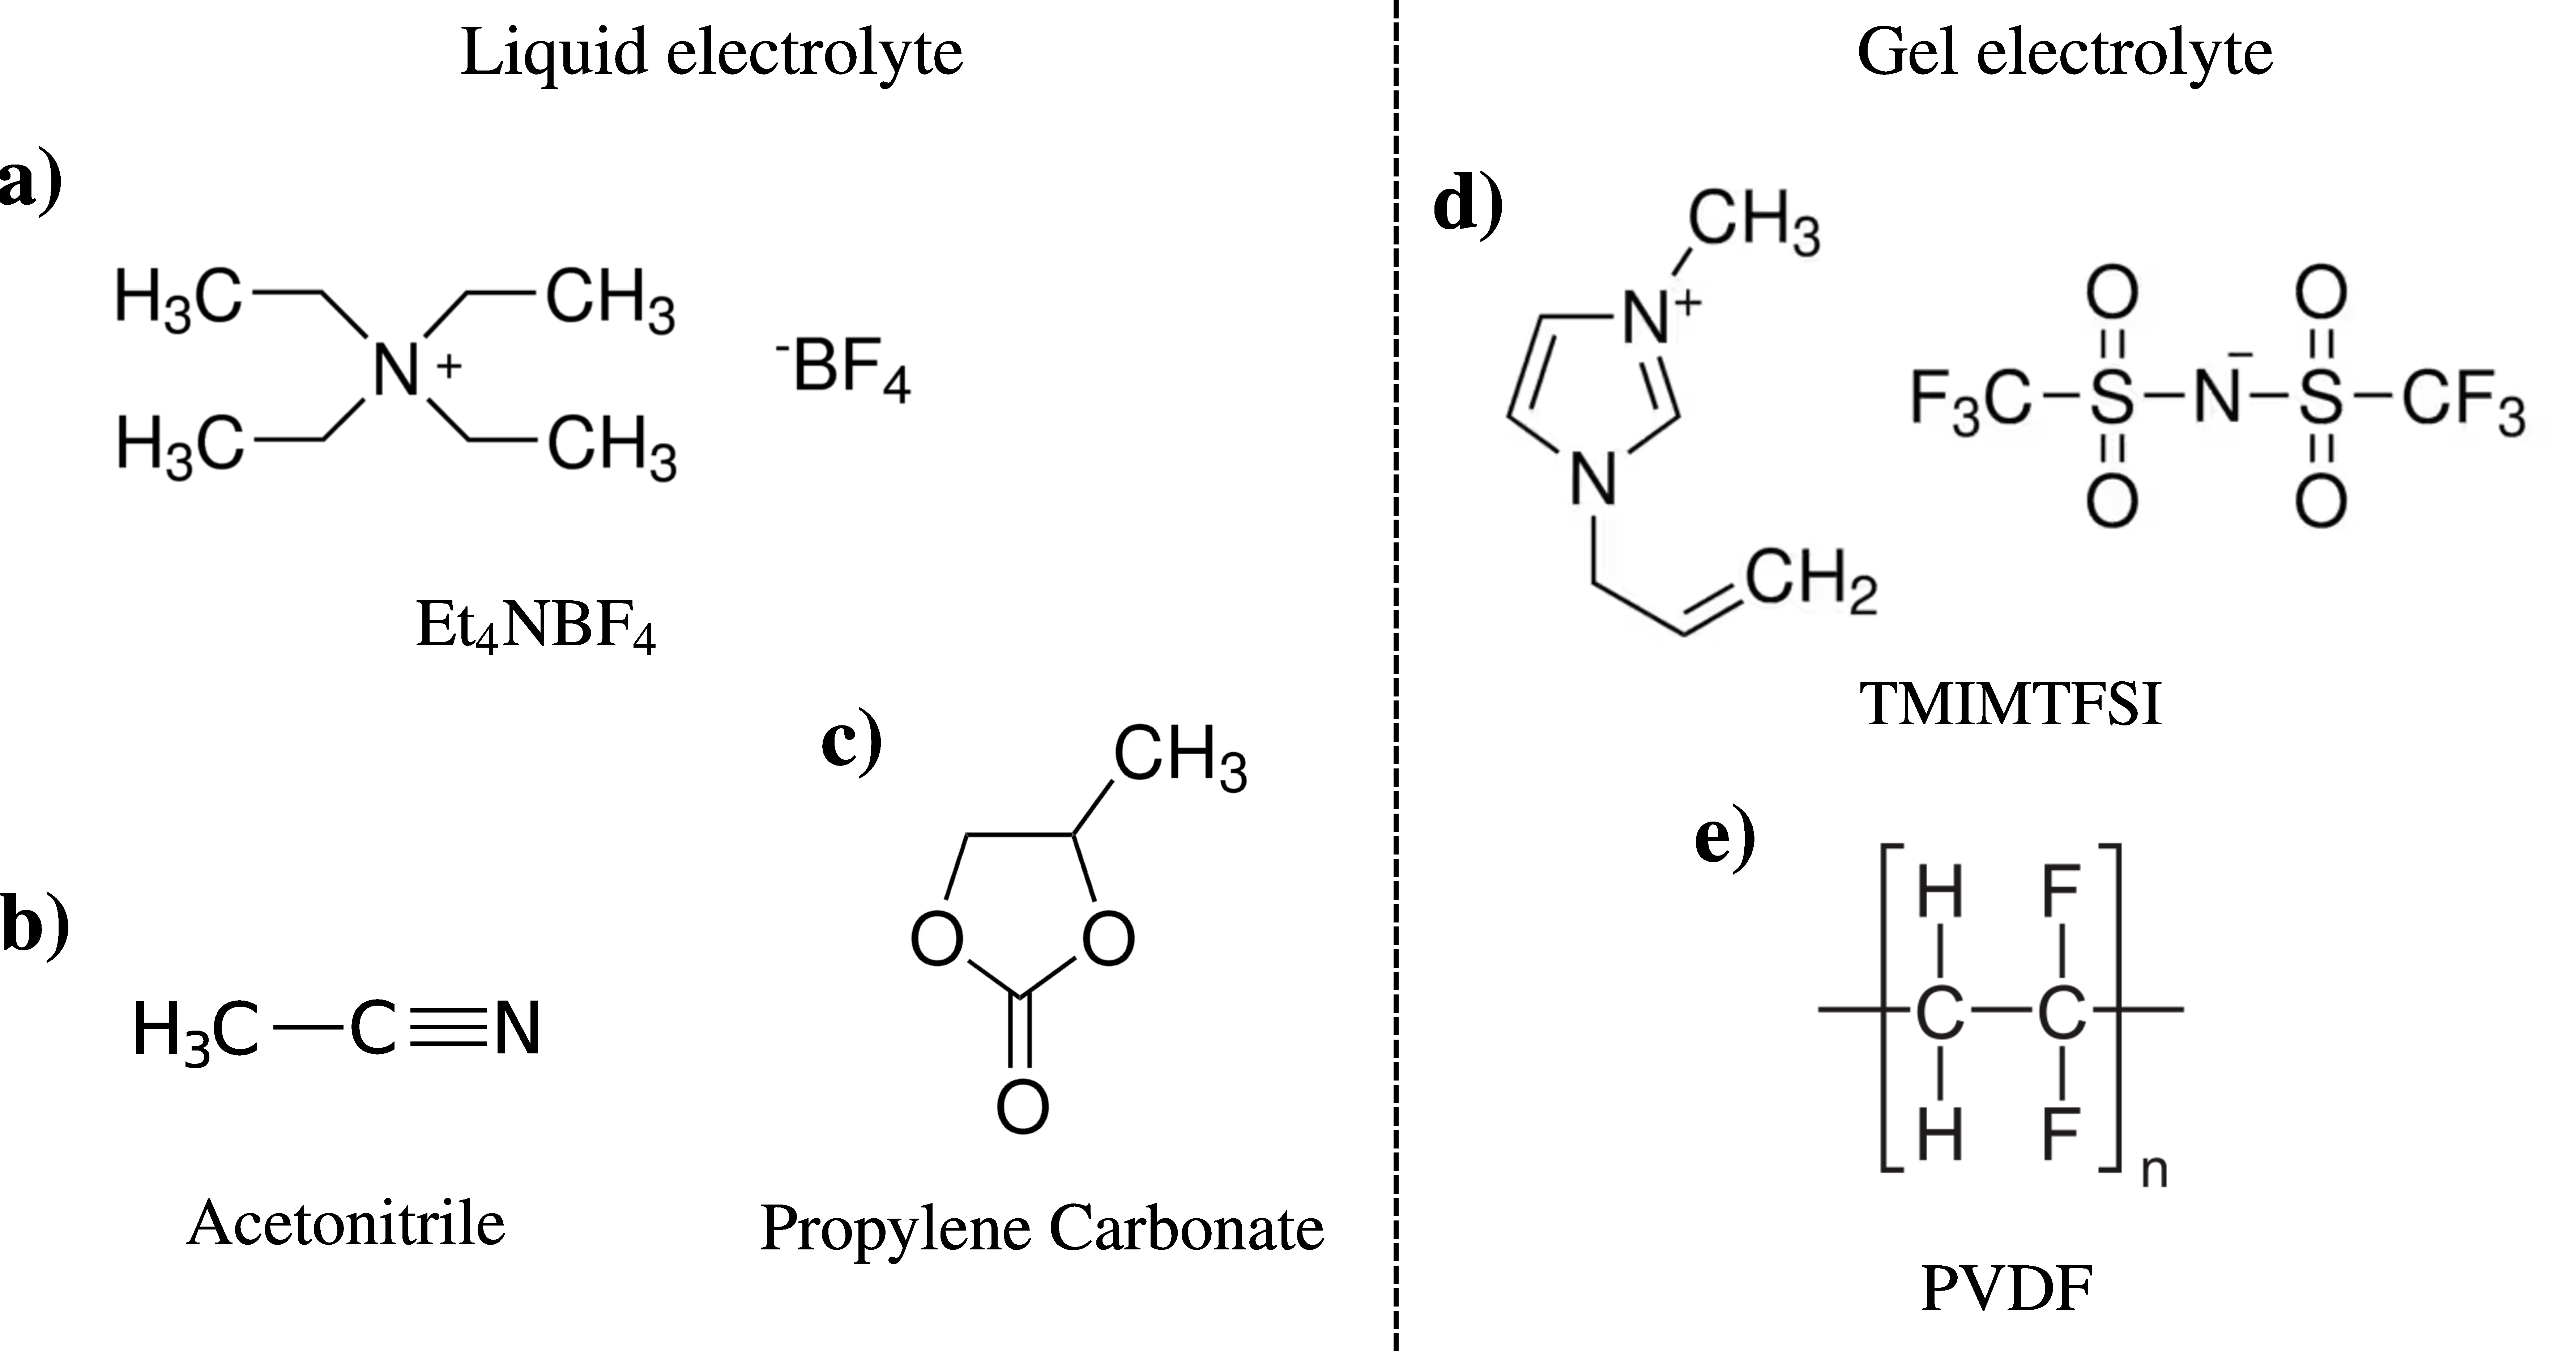
\includegraphics[width=0.9\textwidth]{./electrochemistry/figures/materials/electrolytes.pdf}
	\caption{Ionic salt (ET$_4$NBF$_4$, a) and the corresponding solvents (Acetonitrile (b) and Propylen Carbonate~(c) for liquid electrolytes. Ionic liquid (TMIMTFSI, d)) and polymer matrix (PVDF, e)) for the gel electrolyte.}
	\label{fig:electrolytes}
\end{figure}

\subsubsection{Liquid Electrolyte}
Tetraetylammonium tetrofluoroborate (Et$_4$NBF$_4$, Figure~\ref{fig:electrolytes}~a) is a crystalline salt that dissociates into a Et$_4$N$^-$ cation and a BF$_4^-$ anion in polar solvents such as Acetonitrile (CH$_3$CN, Figure~\ref{fig:electrolytes},b) and Propylene Carbonate (C$_4$H$_6$O$_3$, Figure~\ref{fig:electrolytes},c). Et$_4$NBF$_4$ is a small molecule with a relatively high dissociation energy, so the solvents have high dielectric constants ($\varepsilon\approx40$ for Acetonitrile and $\varepsilon\approx64$ for Propylene Carbonate). Propylene Carbonate has higher density than Acetonitrile, has higher viscosity and is less volatile. A 100~mM solution of Et$_4$NBF$_4$ in Acetonitrile or in Propylene Carbonate ensures sufficient ionic transport for the organic electrochemical cells described later in this section.

\subsubsection{Polymer-based Gel Electrolyte}
The use of ionic liquids and the suitable polymer matrix allows for fabrication solid-state electrolytes that are used for making organic electrochemical neurons~\cite{Harikesh2022} and solid-state Li batteries~\cite{Pang2021}. PVDF (Figure~\ref{fig:electrolytes}~e) was used as a polymer matrix. TMIMTFSI (Figure~\ref{fig:electrolytes}~d) was the ionic liquid. The polymer grains were dissolved in Chloroform at 80~$^{\deg}$C and the ionic liquid was mixed in at a ratio $1:4:20$ (polymer : ionic liquid : solvent). The polymer electrolyte was used to manufacture an all-polymer organic radical battery described later in this section.

\section{Organic Electrode Materials}
\label{sec:ORB_materials}
ORB based on redox polymers containing stable radicals~\cite{nakahara2002_cpl} have been shown to compete with or even outperform  conventional Li based batteries in terms of power densities~\cite{IWASA2007} with the additional benefit of being free from rare precursors, inheriting mechanical properties of plastics and electrical properties of semiconductors~\cite{friebe2017_topcurrchem,Casado2021,Goujon2021}. Advanced molecular design techniques allow for tuning of the electrochemical properties of the redox polymers~\cite{Janoschka2017}, that brings in a rich variety of organic energy storage materials~\cite{Xie2021,Vereshchagin2022,Janoschka2017a} and creates a large room for their optimization. 

\par
\subsection{TEMPO}
TEMPO (2,2,6,6-tetramethylpiperidine-1-oxyl) shown in Figure~\ref{fig:molecules}~a) is a small molecule and a stable radical that can undergo a fast and reversible redox reaction between TEMPO$^\bullet$ and TEMPO$^+$~\cite{Wang2019}, with an electron self-exchange rate constant of $k_{ex}\approx10^{6-8}$ M$^{-1}$~s$^{-1}$~\cite{Chatgilialoglu2012}. TEMPO is an inexpensive organic compound~\cite{Vereshchagin2022} produced from acetone with liquid ammonia, hydrazine and peroxide~\cite{Casado_2021_book}. TEMPO radicals are widely used as spin labels in the studies of biological systems with electron spin resonance~\cite{Bordignon2017}, because the unpaired electron of TEMPO$^\bullet$ has a well defined spectral signature that changes when the local environment of a TEMPO fragment changes. TEMPOL is a TEMPO with an OH group. It is soluble in many organic solvents and forms crystals. Solutions of TEMPOL with various concentrations can be used for the reference spectroscopic measurements, as by varying the concentration the strength of inter-spin interactions between the neighboring radicals can be adjusted.

\begin{figure}[h]
\center
	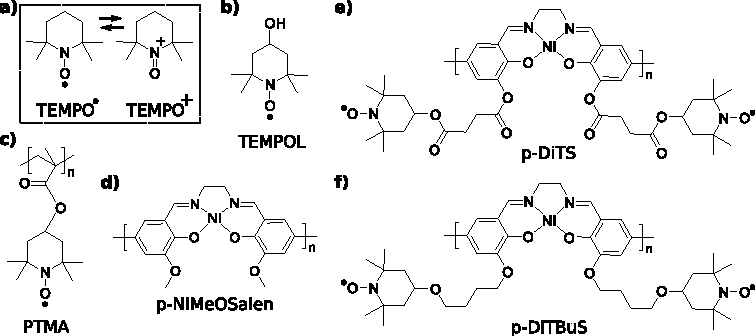
\includegraphics[width=1\textwidth]{./electrochemistry/figures/materials/molecules.pdf}
	\caption{Chemical structures of the molecular fragments and polymers that were used for making a battery cathode containing stable nitroxide radicals.}
	\label{fig:molecules}
\end{figure}



Redox conductive conjugated polymers containing TEMPO redox groups, as pDiTBuS (poly-di-TEMPO-Butyl-Salen) shown in Figure~\ref{fig:Figure_1}, demonstrate particularly promising energy and power densities~\cite{Vereshchagin2020}. The pDiTBuS was designed as a cathode material: it is oxidized when the electrochemical cell containing this material is charged. A film of pDiTBuS comprises a high concentration of redox active stable nitroxyl radicals attached to a conjugated polymer backbone that interconnects them as a molecular wire. Such system can be viewed as a highly disordered molecular hole-transporting semiconductor (the poly-NiSalen backbone) that contains a large amount of hole traps (TEMPO groups) attached to it with butyl linkers. When the film is reduced (discharged), the TEMPO groups are in the radical state and act as unfilled traps. Upon oxidation (charging), the TEMPO fragments lose an unpaired electron and acquire a positive charge, so the traps are being filled with holes. The reversible redox reaction in the pDiTBuS film is demonstrated in a cyclic voltammogram shown in Figure~\ref{fig:CV_DiTBuS}, c) and in the equal charging and discharging capacity of the film in Figure~\ref{fig:GCD_DiTBuS}, c).

\par
While active electrode materials with nitroxide radicals as redox-active groups are ideally suited for organic radical batteries (ORBs) that exhibit high power densities, the broad application of most nitroxide-based materials is limited by their moderate electrical properties. A promising route towards overcoming the conductivity problem is the use of polymers that combine radical-containing moieties and a conductive backbone. This strategy was successfully followed in a number of studies focusing on different polymers~\cite{oyaizu2015_polymerjournal, bahaceci2013_jpowersources, katsumata2006_mrc, xu2014_electact, aydin2015_jsoistatelect, schwartz2018_synthmet}. The standard redox potential of the NiSalen molecular backbone ($E_{1/2}^B$ in the middle of the peaks B and B$^\prime$ in Figure~\ref{fig:CV_DiTBuS}) lay close to the standard redox potential of the attached nitroxide charge-bearing fragments ($E_{1/2}^A$ in the middle of the peaks A and A$^\prime$ in Figure~\ref{fig:CV_DiTBuS}) - that ensures an efficient charge transport between the charge-bearing fragments and the conductive backbone and allows for very high charge and discharge rates up to 3000~C~\cite{Vereshchagin2020,Kulikov2022}.

\subsection{PTMA}
A simple organic radical polymer containing TEMPO is poly-TEMPO-methacrylate) (PTMA, Figure~\ref{fig:molecules}~c). The polymer backbone of PTMA consists of single C-C bonds and therefore is not conductive, so the transport of charge in a PTMA film has to be mediated by adding conductive mesh such as activated carbon. When mixed with conductive carbon additive, PTMA has become a standard cathode material for ORBs and Li-ORBs, providing a discharge cell voltage of V$_{OC}=3.5$~V (with a Li anode) and a theoretical discharge capacity of $C_{theo}=111$~mAh/g~\cite{Daniel2023_Multimodal}. PTMA is soluble in acetonitrile (AN), chloroform (CF), tetrahydrofurane and dichlormethane. It is claimed to be insoluble in toluene, ethers, carbonates, and alcohols, however it becomes gel-like with some of these solvents~\cite{DOM}.

\subsection{NiSalen}
The molecular backbone of a redox conductive polymer has to conduct electric charge. A NiSalen molecule shown in Figure~\ref{fig:molecules}~d) is a Schiff complex of Ni that has a conjugated path through it. p-NiMeoSalen is polymerized NiSalen with two methoxy groups, that forms the conductive backbone of the corresponding RCPs in e) and f). The pNiSalen backbone is redox active and can store up to 2 positive charges per monomer unit~\cite{Dmitrieva2018}. The conductivity of p-NiSalen depends on its oxidation state. The oxidized polymer has higher conductivity due to a higher concentration of holes~\cite{Dmitrieva2018}. Upon oxidation of a polymeric NiSalen, the formation of positive polarons and bipolarons was observed in it with UV-Vis and EPR spectroscopy~\cite{Dmitrieva2018}, that suggests p-NiSalen is a p-type molecular semiconductor.


\subsection{Poly-Di-TEMPO-Salens}
Redox conductive conjugated polymers containing TEMPO (2,2,6,6-tetramethylpiperidine-1-oxyl) redox groups, as pDiTS~\cite{Vereshchagin2020,Kulikov2022} (poly-Di-Tempo-Salen) and pDiTBuS~\cite{Kulikov2023} (poly-di-TEMPO-Butyl-Salen) shown in Figure~\ref{fig:molecules} e) and f), demonstrate particularly promising energy and power densities with charging rates upto 3000~C and gravimetric capacity upto 91.5~mAh~g$^{-1}$ for pDiTS~\cite{Vereshchagin2020} and upto 75~mAh~g$^{-1}$ for pDiTBuS~\cite{Kulikov2023}. pDiTS and pDiTBuS have similar molecular structures, except for pDiTBuS has no oxygens in the linkers that connect the backbone to the TEMPO fragments, which has led to its higher electrochemical stability and a more efficient electro-polymerization, that allows for growing thicker films. pDiTS is a charge storage material that consists of TEMPO redox active molecular fragments~\cite{Vereshchagin2022,jeschke2012_annrevphyschem,Halbmair2016} interconnected by a redox conductive conjugated NiSalen backbone~\cite{Vereshchagin2020,Dmitrieva2018}. DiTS and DiTBuS monomers were synthesized in the Levin group at the Saint-Petersburg State University.\\
pDiTS was designed as a cathode material: it is oxidized when the electrochemical cell containing this material is charged. A film of pDiTBuS comprises a high concentration of redox active stable nitroxyl radicals attached to a conjugated polymer backbone that interconnects them as a molecular wire. Such system may be viewed as a highly disordered molecular hole-transporting semiconductor (the poly-NiSalen backbone) that contains a large amount of hole traps (TEMPO groups) attached to it with butyl linkers. When the film is reduced (discharged), the TEMPO groups are in the radical state and act as unfilled traps. Upon oxidation (charging), the TEMPO fragments lose an unpaired electron and acquire a positive charge, so the traps are being filled with holes~\cite{Kulikov2023}.

\begin{figure}[h]
\center
	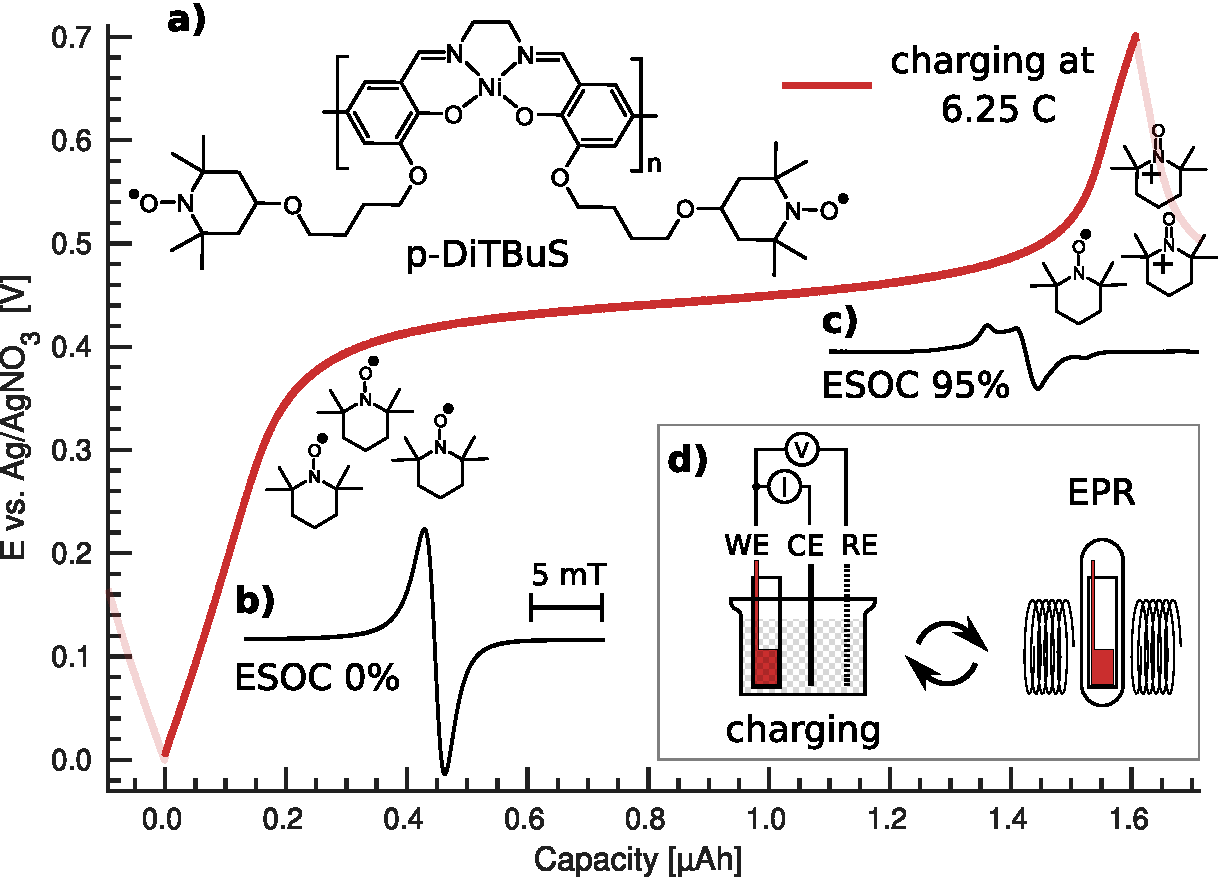
\includegraphics[width=0.7\textwidth]{./introduction/figures/Figure_1.pdf}
	\caption{Galvanostatic charge-discharge curve for a pDiTBuS cathode film at 10~$\muup$A (6.25~C), chemical structure of pDiTBuS (a), normalized cwEPR spectral signatures for reduced (b) and oxidized (c) states. Scheme of the ex-situ EPR measurement on the pDiTBuS half cell (d).}
	\label{fig:Figure_1}
\end{figure}



\begin{figure}[!h]
\center
	\includegraphics[width=0.7\textwidth]{./electrochemistry/figures/materials/DiTS_SEM.png}
	\caption{Scanning electron microscope images of a pDiTS film in a reduced (a) and oxidized (b) states, image adapted from Ref.~\cite{Vereshchagin2020}.}
	\label{fig:Figure_1}
\end{figure}


\subsection{Electro-polymerization of TEMPO-Salens}
\begin{figure}[!h]
\center
	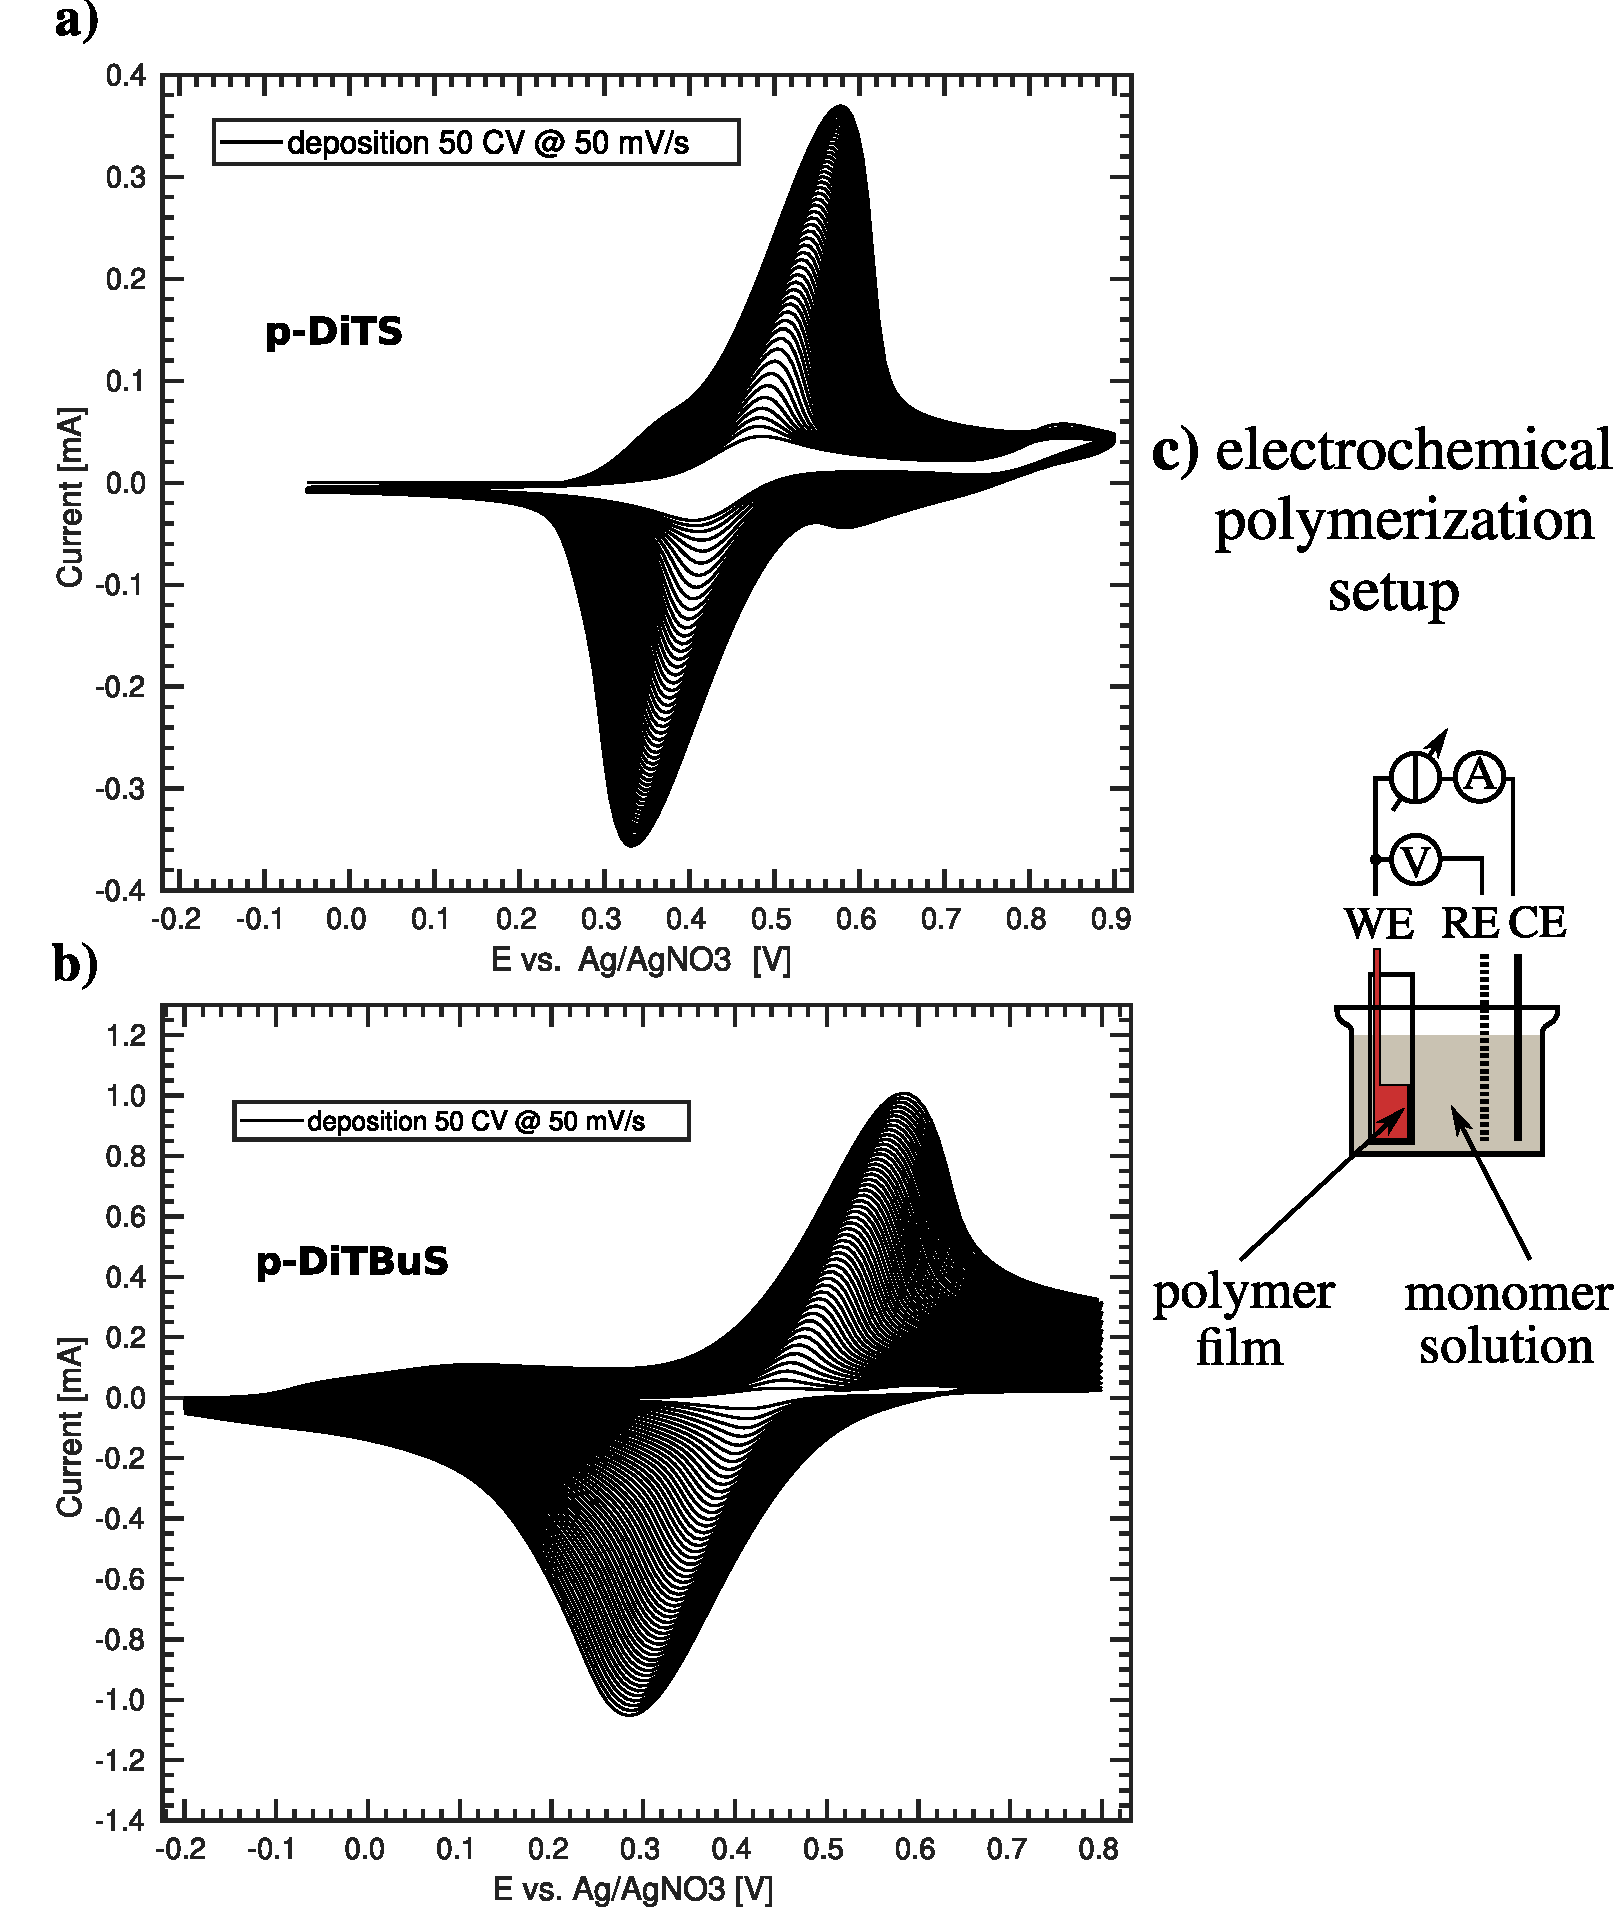
\includegraphics[width=0.65\textwidth]{./electrochemistry/figures/DITBUS_DEPO.pdf}
	\caption{Deposition of TEMPO-Salen films with cyclic electrochemical polymerization from 1~mM monomer solutions in the 10~mM Et$_4$NBF$_4$ electrolyte at 50~mVs$^{-1}$ and 50 deposition cycles. a): pDiTS, b): pDiTBuS. c) setup for electrochemical polymerization}
	\label{fig:DITBUS_DEPO}
\end{figure}

The process of polymerization is connecting multiple monomer units of one sort to a continuous molecular chain. A polymerization of redox active molecules, such as NiSalen monomer fragnents, can be done electrochemically with the setup shown in Figure~\ref{fig:electropolymerization_reaction}. A three-electrode cell is made with a 10~mM solution of NiSalen in the electrolyte. By applying a positive voltage between the WE (Au) and the CE (Pt), NiSalen molecules are adsorbed to the surface of the WE and oxidized. Oxidation of NiSalen leads to a formation of a positive radical in the ring of the NiSalen that can be seen as the opening of the ring, as shown in the diagram in Figure~\ref{fig:electropolymerization_reaction}. The oxidized, open ring attracts the next NiSalen molecule from the solution, then the positive radical is transferred from the ring to the attracted molecule through the conjugated network and the two molecules form a bond~\cite{Koshika_2009}. The reaction repeats until the conductivity of the film allows for efficient transfer of the positive radical to its outer surface, so a pNiSalen film is grown on the WE surface~\cite{Apraksin2021,Novozhilova_2009Vereshchagin2020}.\\ 
\par
The electrochemical polymerization of a TEMPO-Salen cannot be done in the same way as for pNiSalen because of the electrical screening effect of the charge-bearing TEMPO radicals that tend to charge together with NiSalen and form a Coulombic schield that repells the TEMPO-Salen fragments in the solution~\cite{Vereshchagin2020}. To discharge the TEMPO fragments, the growing film has to be periodically discharged, so a cycling voltage is applied to perform a cyclic polymerization of pDiTS and pDiTBuS films~\cite{Vereshchagin2020,Kulikov2023}. The effect of charging is also pronounced in the polymerization of NiSalen films due to their charge-storing ability, so both pNiSalen and poly-TEMPO-Salen films are grown with cycling polymerization.\\

\begin{figure}[!ht]
\center
	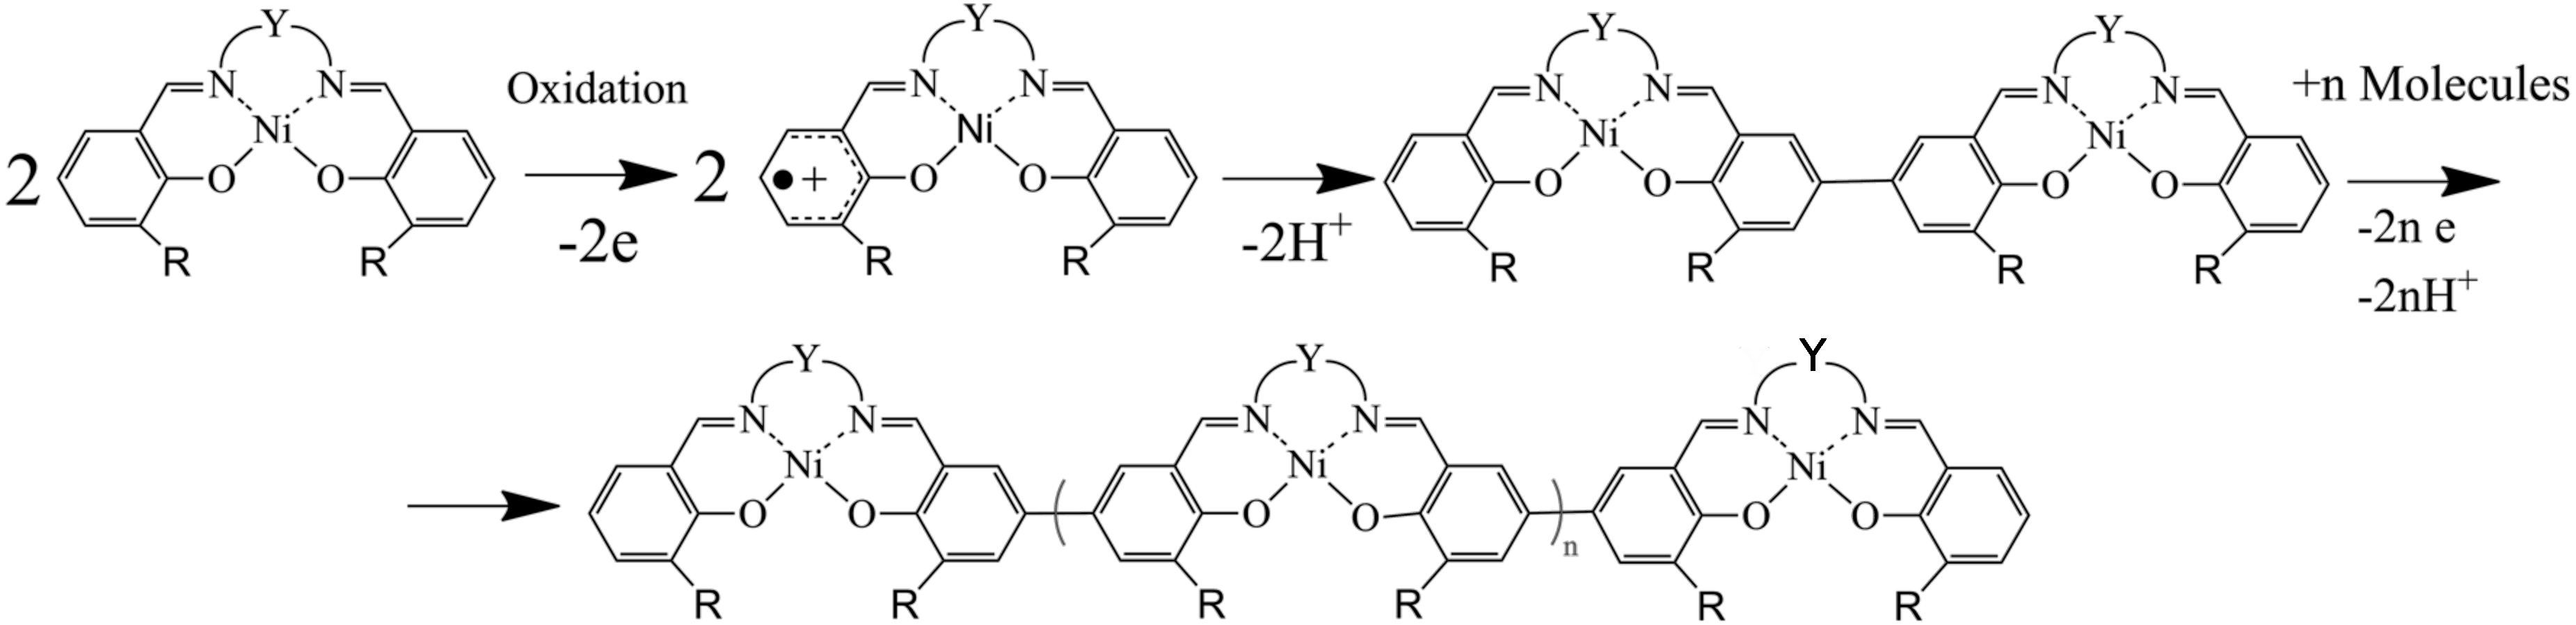
\includegraphics[width=1\textwidth]{./electrochemistry/figures/electropolymerization_reaction.pdf}
	\caption{A scheme of a two-step cyclic electropolymerization of NiSalen containing electrochemically inactive side groups (R). First, two monomers are oxidized upon application of a positive potential to the cell containing the monomer solution, that induces a cation (hole) in their phenyl rings. The oxidized monomers create a bond by sharing their cations. When the potential is ramped down, the holes are withdrawn from the radicals and they remain connecting by forming a C-C bond instead of closing the bond in their rings.}
	\label{fig:electropolymerization_reaction}
\end{figure}


\section{Ex Situ Electrochemistry}
\label{sample_fab_2}
The pDiTBuS film was brought to the desired oxidation state by galvanostatic discharging with a current of 10~$\muup$A in a three-electrode electrochemical cell in a 5~ml beaker with the electrodes and the electrolyte described above.
Each potential of the film was reached by first fully charging the cell to 700~mV and then discharging it to the desired potential (labeled points in Figure~\ref{fig:Figure_S3}). When the desired potential was \ik{reached}, the output relay of the potentiostat was opened so that no current went through the cell after charging. The substrate with the WE and the pDiTBuS film was removed from the charging cell, placed in a 5~mm OD quartz EPR tube, evacuated down to $<5\times10^{-3}$~mbar, filled with He up to a pressure of 500-600 mbar, then flame sealed with a H$_2$/O$_2$ burner.

\begin{figure}[!ht]
\center
	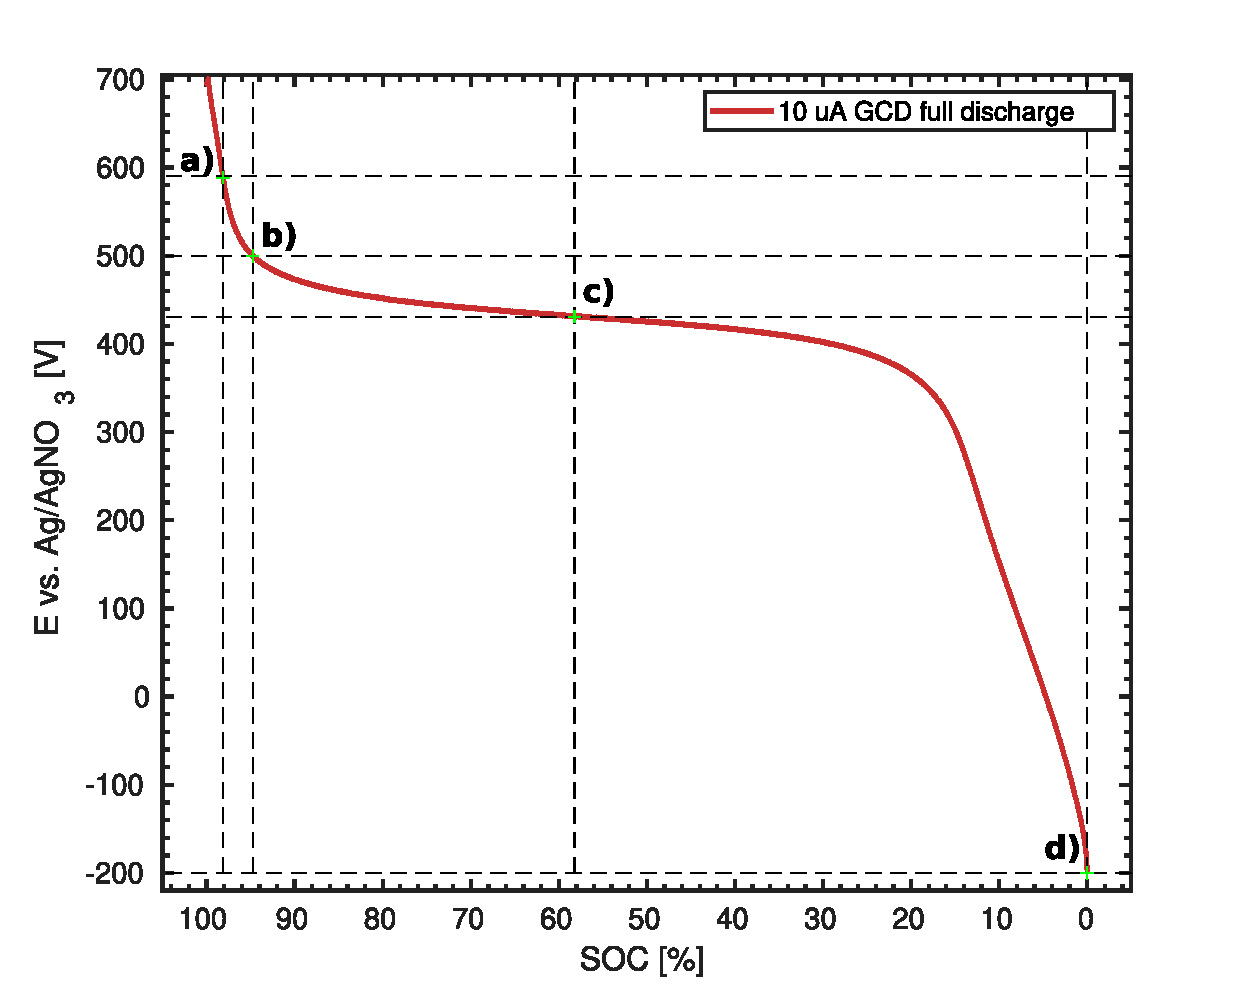
\includegraphics[width=0.85\textwidth]{./pulse/figures/Figure_S3}
	\caption{Initial galvanostatic discharge curve for the pDiTBuS film with the redox potentials described in the main text. Since the film has lost 12\% of its capacity during the temperature cycling, the SoC determined from the potentials mapped to the initial curve are lower than the SoC determined from the individual discharge curves (given in brackets). The SoC values corresponding to the initial (individual) discharge curve are a): SoC~98~(98)\%, b): SoC~\ik{94~(96)}\%, c): SoC~57(65)\%, d): SoC~0(0)\%. (Dis-)charging current: 10~$\muup$A, charging rate: 6.25~C. After this initial discharging, the pDiTBuS film has undergone 10 charge-discharge cycles and 4 temperature cycles.}
	\label{fig:Figure_S3}
\end{figure}

\begin{figure}[!ht]
\center
	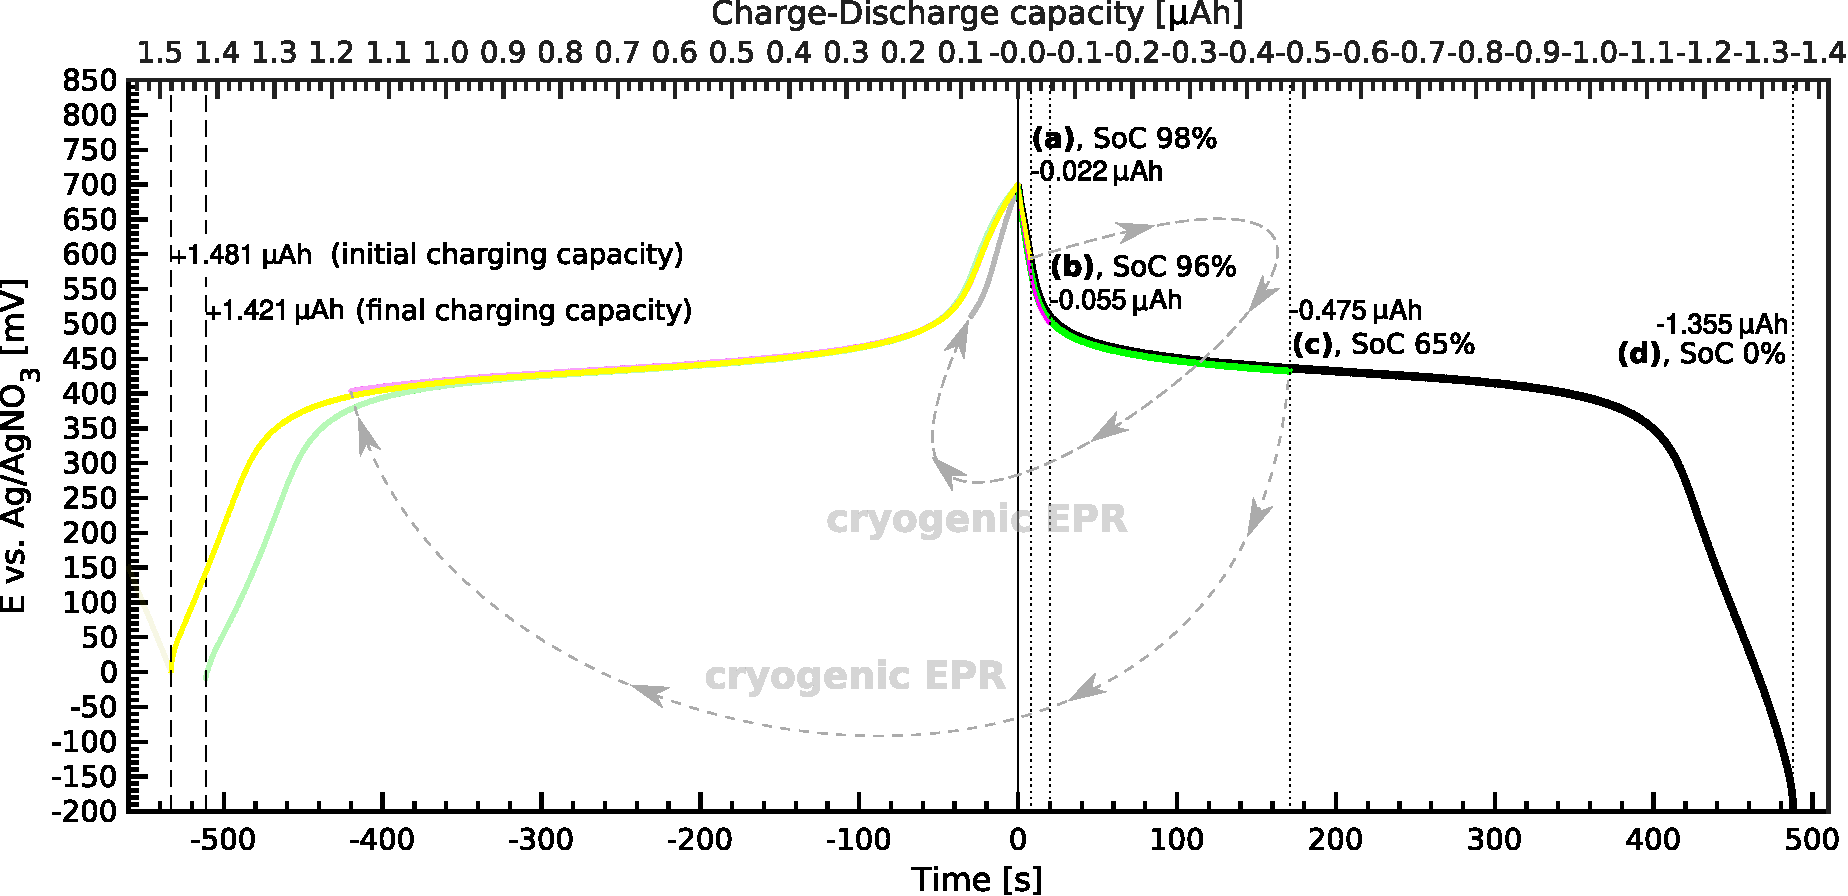
\includegraphics[width=1\textwidth]{./pulse/figures/Figure_S27}
	\caption{\ik{Calculation of the number of withdrawn electrons from a pDiTBuS film for the four states of charge. At negative times the pDiTBuS film is charged, corresponding to the withdrawal of electrons from the film. At positive times the film is discharged. The number of transferred electrons during discharging is determined from the four overlaid galvanostatic discharge curves (a-d).}}
	\label{fig:Figure_S27}
\end{figure}

\ik{
After reaching the fully charged state with 10~$\muup$A (by $t=0$ in Figure~\ref{fig:Figure_S27}), a 10~$\muup$A discharge current was applied to reach the four states of charge considered in this study (a-d in Figure~\ref{fig:Figure_S27} and in Figure~\ref{fig:Figure_S3}). Initially, the full charging capacity of the film was 1.48~$\muup$Ah~$=5.11$~\ik{m}C (3.29e+16 electrons withdrawn upon the full charging). The charging capacity has decreased by 0.06~$\muup$Ah ($4\%$) after the four temperature cycles between 300~K and 5~K during the cryogenic EPR measurements.\\
}
\newpage
\ik{
From the quantitative analysis of the GCD for each SoC, we calculate the number of elementary charges that are transferred to the film (withdrawn from the film) upon charging (discharging). The GCD and the calculated values of the transferred charge are shown in Figure~\ref{fig:Figure_S27}. During the full discharge from +700~mV down to -200~mV the pDiTBuS film has gained a total charge of 1.355~$\muup$Ah=4.88~\ik{m}C (d), corresponding to 3.01e+16 electrons that had been transferred to the film.)
}
\ik{ 
The considered SoC correspond to discharging by $0.020\pm0.005~\muup$Ah (Figure~\ref{fig:Figure_S27}~a, $(5\pm1)\times10^{14}$ electrons injected), $0.060\pm0.005~\muup$Ah (Figure~\ref{fig:Figure_S27}~b, $(1.4\pm0.1)\times10^{15}$ electrons injected), $0.480\pm0.005~\muup$Ah (Figure~\ref{fig:Figure_S27}~c, $(1.07\pm0.01)\times10^{16}$ electrons injected) and $1.360\pm0.005~\muup$Ah (Figure~\ref{fig:Figure_S27}~d, $(3.05\pm0.01)\times10^{16}$~electrons injected). The SoC values determined from the respective potentials are different when mapped to the initial discharge curve in Fig.~\ref{fig:Figure_S3} and when considering the individual discharge curves in Fig.~\ref{fig:Figure_S27}, as the film was gradually losing its capacity during the temperature cycling, so the discharge curves were reaching the considered potentials at shorter times, leading to a lower Coulomb counting, lower discharge capacity and therefore a lower SoC.}




\subsection{Electrochemical Cells with Solid Electrolyte}
The electrolyte based on an ionic liquid incorporated in a gel-like polymer matrix has sufficient ionic mobility and diffusion to penetrate the pDiTBuS and pNiSalen surface and allow for partial charging and discharging of the battery electrodes. TEMPO radicals were shown to undergo a redox reaction in ionic liquids with a slightly changed redox potential of the TEMPO$^{\bullet}$-TEMPO$^+$ reaction~\cite{Golovisnina2023}.

\begin{figure}[h]
\center
	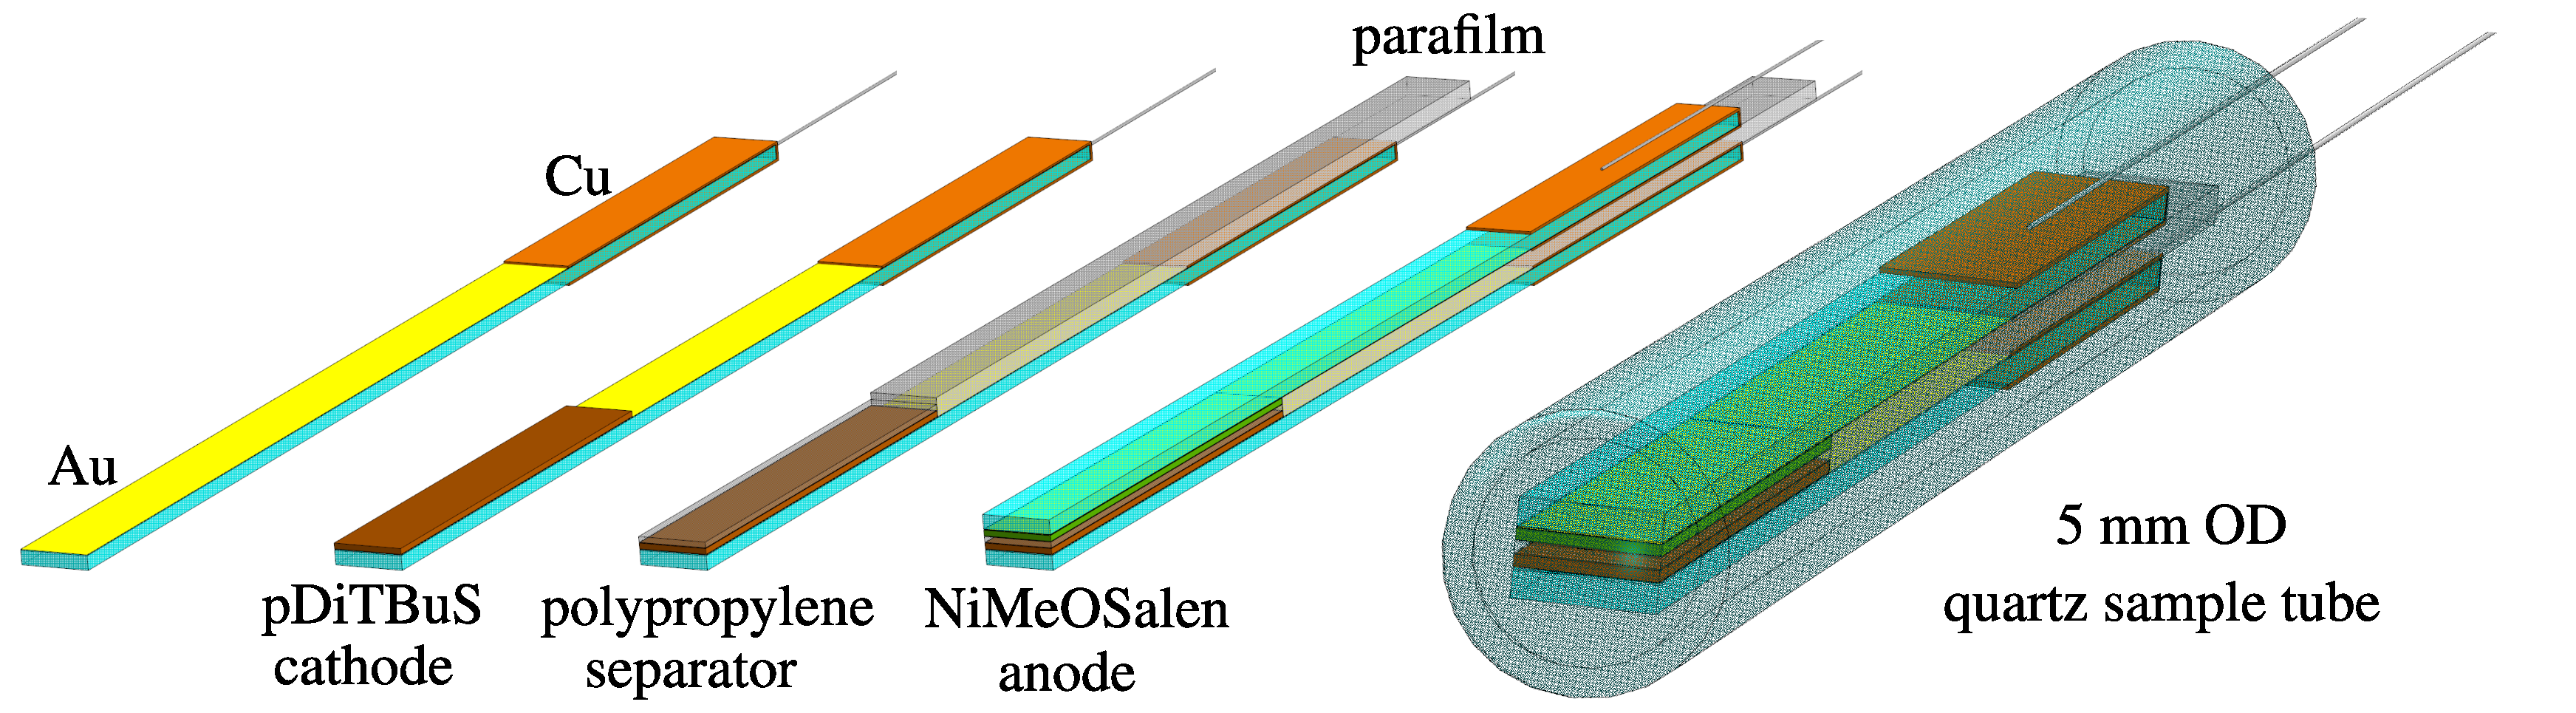
\includegraphics[width=1\textwidth]{./operando_epr/figures/sandwich/sandwich.pdf}
	\caption{Organic radical battery made with two parallel Au-plated substrates and a polypropylene separator soaked in liquid electrolyte.}
	\label{fig:sandwich_assembly}
\end{figure}



\begin{figure}[h]
\center
	
\includegraphics[width=1\textwidth]{./operando_epr/figures/solid/solid_cell.pdf}
	\caption{All-polymer solid state organic radical battery produced on a 5~$\muup$m interdigitated grid.}
	\label{fig:transistor_battery_assewmbly}
\end{figure}


\begin{figure}[h]
\center
	\includegraphics[width=0.75\textwidth]{./operando_epr/figures/solid/separate_deposition.pdf}
	\caption{Deactivation of the on-substrate CE during the electrodeposition of a pDiTBuS film on the on-substrate WE of a 5~$\muup$m interdigitated grid.}
	\label{fig:transistor_battery_deposition}
\end{figure}

\begin{figure}[h]
\center
	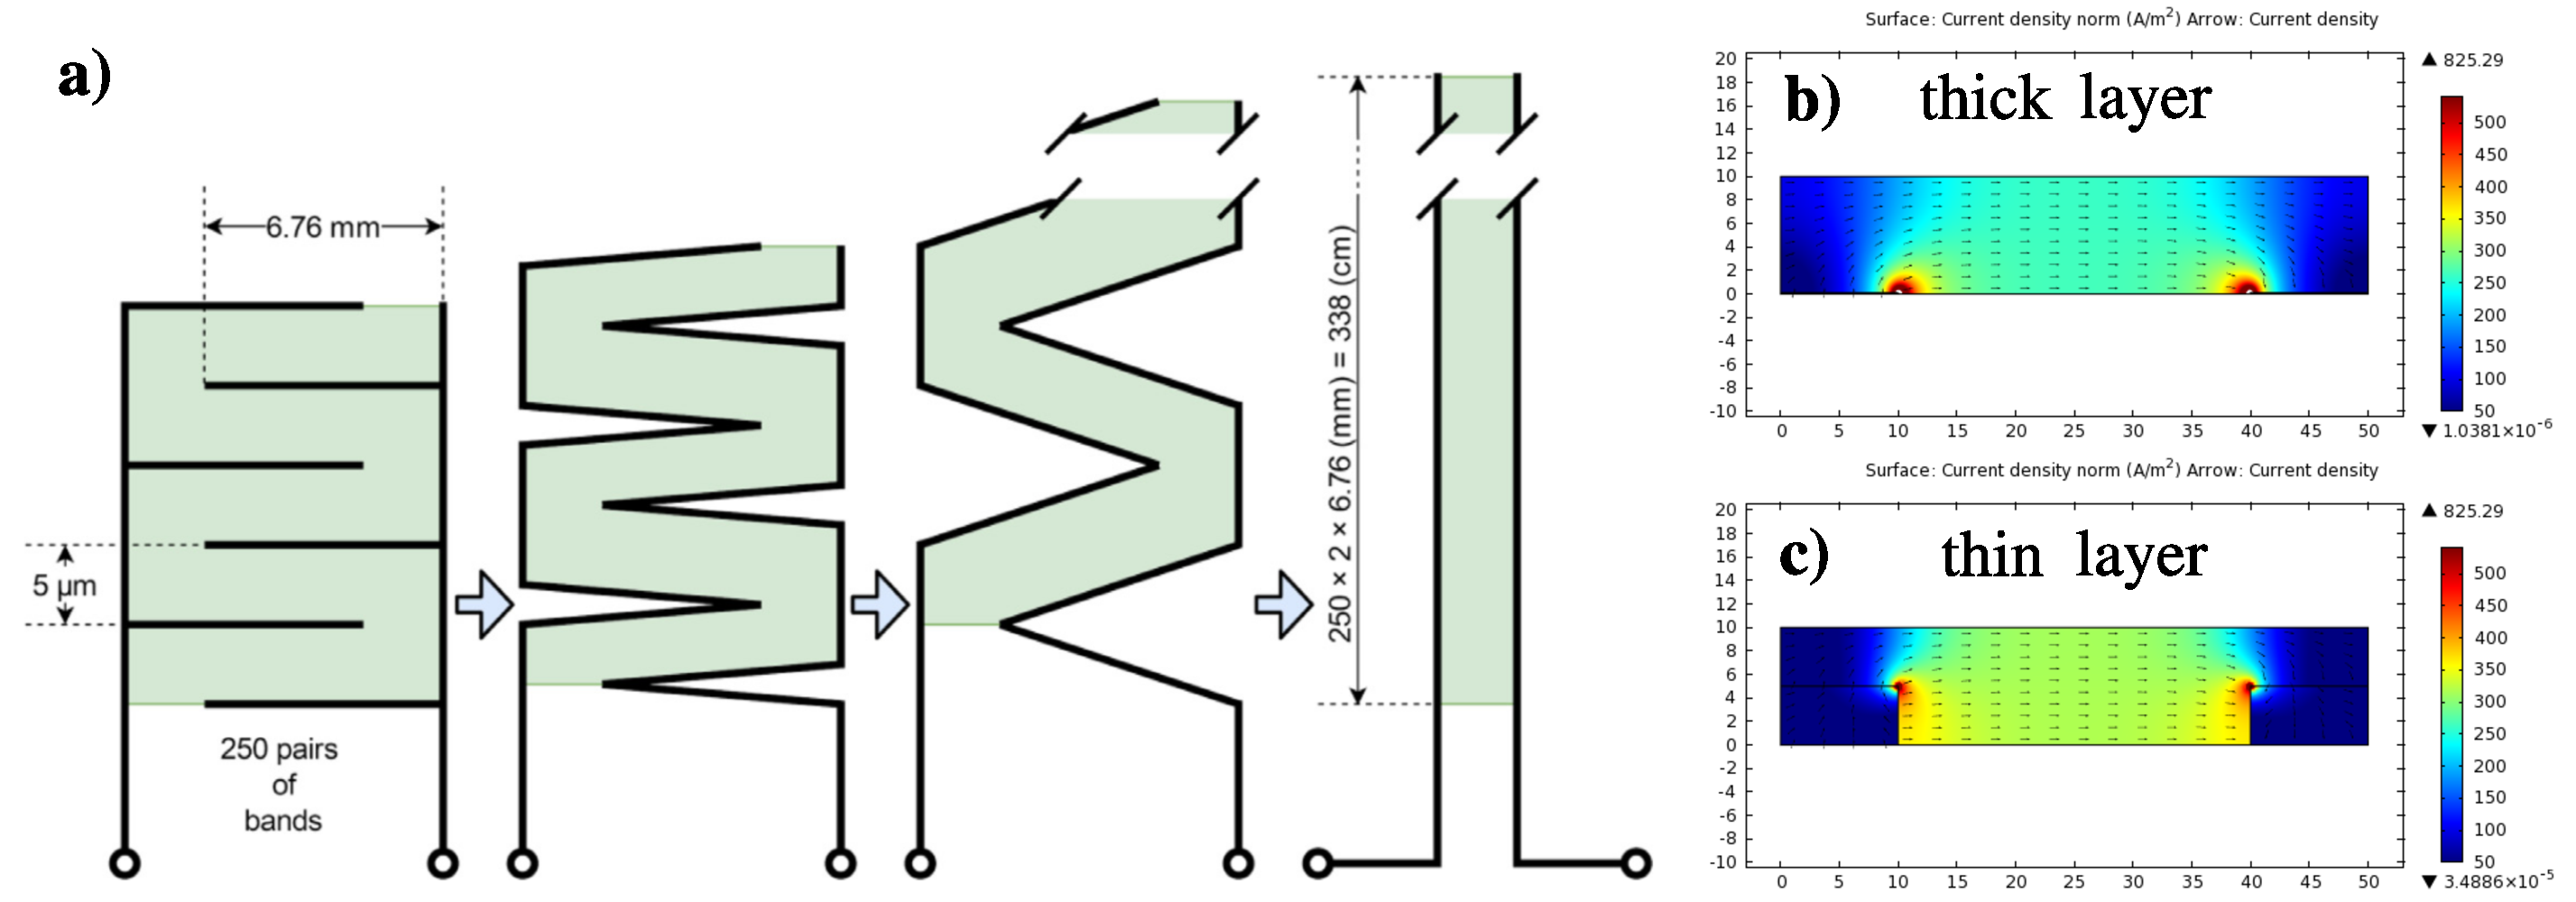
\includegraphics[width=1\textwidth]{./operando_epr/figures/solid/current_density.pdf}
	\caption{Extremely inhomogeneous current density in a closely spaced electrodes of the interdigitated grid. Numerical simulation in Comsol Multiphysics.}
	\label{fig:grid_current_density_sumulation}
\end{figure}


\subsection{Energy Diagram of an Electrochemical Half-Cell}
The transfer of charges in a TEMPO-Salen electrochemical cell can be described in an energy diagram shown in Figure~\ref{fig:band_diagram}. The energy scale of the diagram starts at the vacuum level - the energy of a free electron. The potential energy of an electron in the Au lead in this energy scale is the work function of Au which is 5.1~eV~\cite{Eastman1970}.  
The energy at which an electron in a material can be found with a 0.5 probability is called the Fermi energy.
The Fermi energy of a cathode changes with the SoC of the cell.

The redox potential of TEMPO is 0.812~V vs. SHE~\cite{Zhou2020}.
The absolute potential of the SHE is 4.44~V vs the vacuum level.
The workfunction of Au is 5.1 eV.
The electrochemical window of Acetonitrile is between -3.45~V and +2.35~V vs. SCE (+0.268 V vs SHE)~\cite{Luca2015}.

Electrochemical doping of a semicouducting polymer~\cite{Jacobs2022}:
Charge transfer, ion insertion.
The oxidation and reduction potentials of the ions are separated from the redox potentials of the polymer by several volts, so no charge transfer occurs between the polymer and the electrolyte. The positive charge injected to the polymer from the metal is compensated by the intercalated negative ion. The ionization efficiency in electrochemically doped films is close to 100\%~\cite{Jacobs2022}.\\

\begin{figure}[h]
\center
	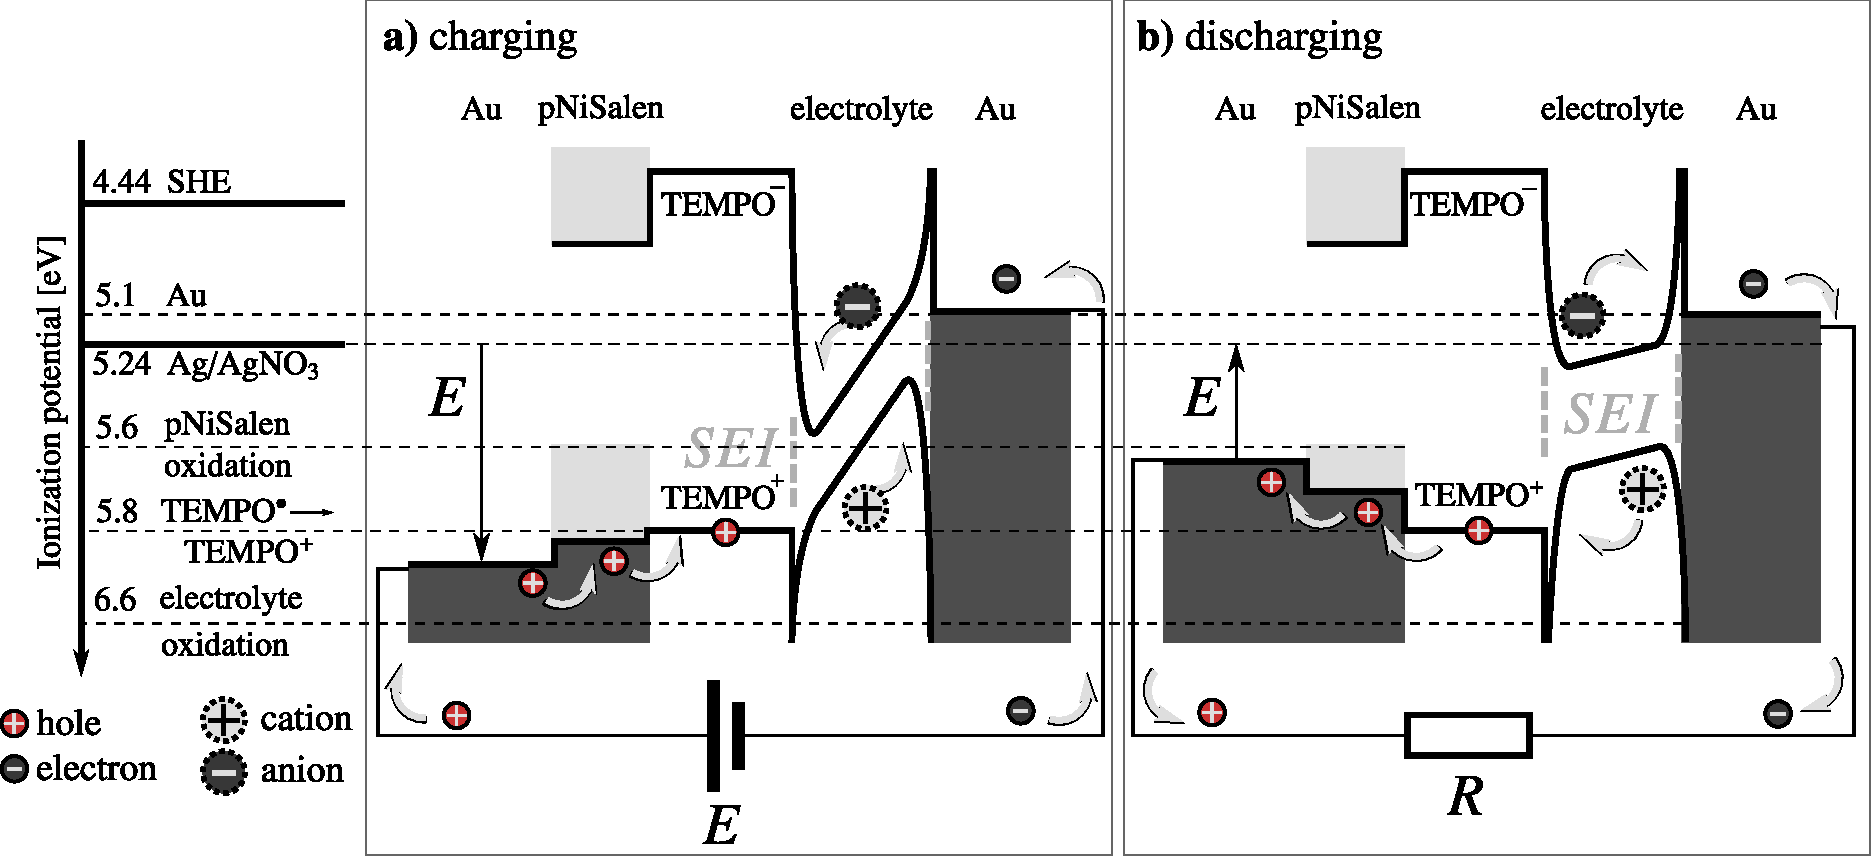
\includegraphics[width=1\textwidth]{./electrochemistry/figures/band_diagram.pdf}
	\caption{Band diagram of a rechargeable electrochemical half-cell with a TEMPO-containing polymer cathode during charging (a) and discharging (b).}
	\label{fig:band_diagram}
\end{figure}

\par
During the charging of a poly-TEMPO-Salen half-cell, its electrochemically active cathode film is being oxidized: positive charges are being injected into it. If the bias potential of the cathode $E$ is higher than the oxidation potential of the polymer (see Figure~\ref{fig:band_diagram}~a)), a positive charge charge is injected to the pNiSalen backbone. The oxidation potential of pNiSalen was adjusted during the molecular synthesis to be close to the oxidation potential of TEMPO$^{\bullet}$, so that the oxidation of the backbone would lead to a simultaneous oxidation of the charge bearing groups~\cite{Vereshchagin2020}. If $E$ increases above the oxidation potential of TEMPO$^{\bullet}$ and the polymer backbone connecting the metal and the TEMPO$^{\bullet}$ fragment is oxidized, the injected hole reaches the TEMPO$^{\bullet}$ fragment and oxidizes it to TEMPO$^+$. The charge transfer process during the charging of the half-cell is shown in Figure~\ref{fig:band_diagram}~a). The oxidation TEMPO$^{\bullet}$ leads to a creation of an electric double layer next to the cathode~\cite{Bhojane2022} of A negative BF4${^-}$ ion is attracted from the electrolyte solution to the positively charged backbone.\\

The hole injected into the polymer backbone propagates in the direction of the Fermi energy gradient within the biased polymer until it encounters the unpaired electron on a TEMPO$^{\bullet}$ group and recombines with it. During the recombination, the hole disappears from the backbone and the electron disappears from the TEMPO$^{\bullet}$. The charge bearing group oxidizes to TEMPO$^+$. This process can be seen as the hole hopping from the backbone to the TEMPO radical. The TEMPO radicals therefore serve as hole traps.


The consequent oxidation of the redox active groups during the biasing of the polymer cathode is shown in Figure~\ref{fig:biasing_charging}.

\begin{figure}[!ht]
\center
	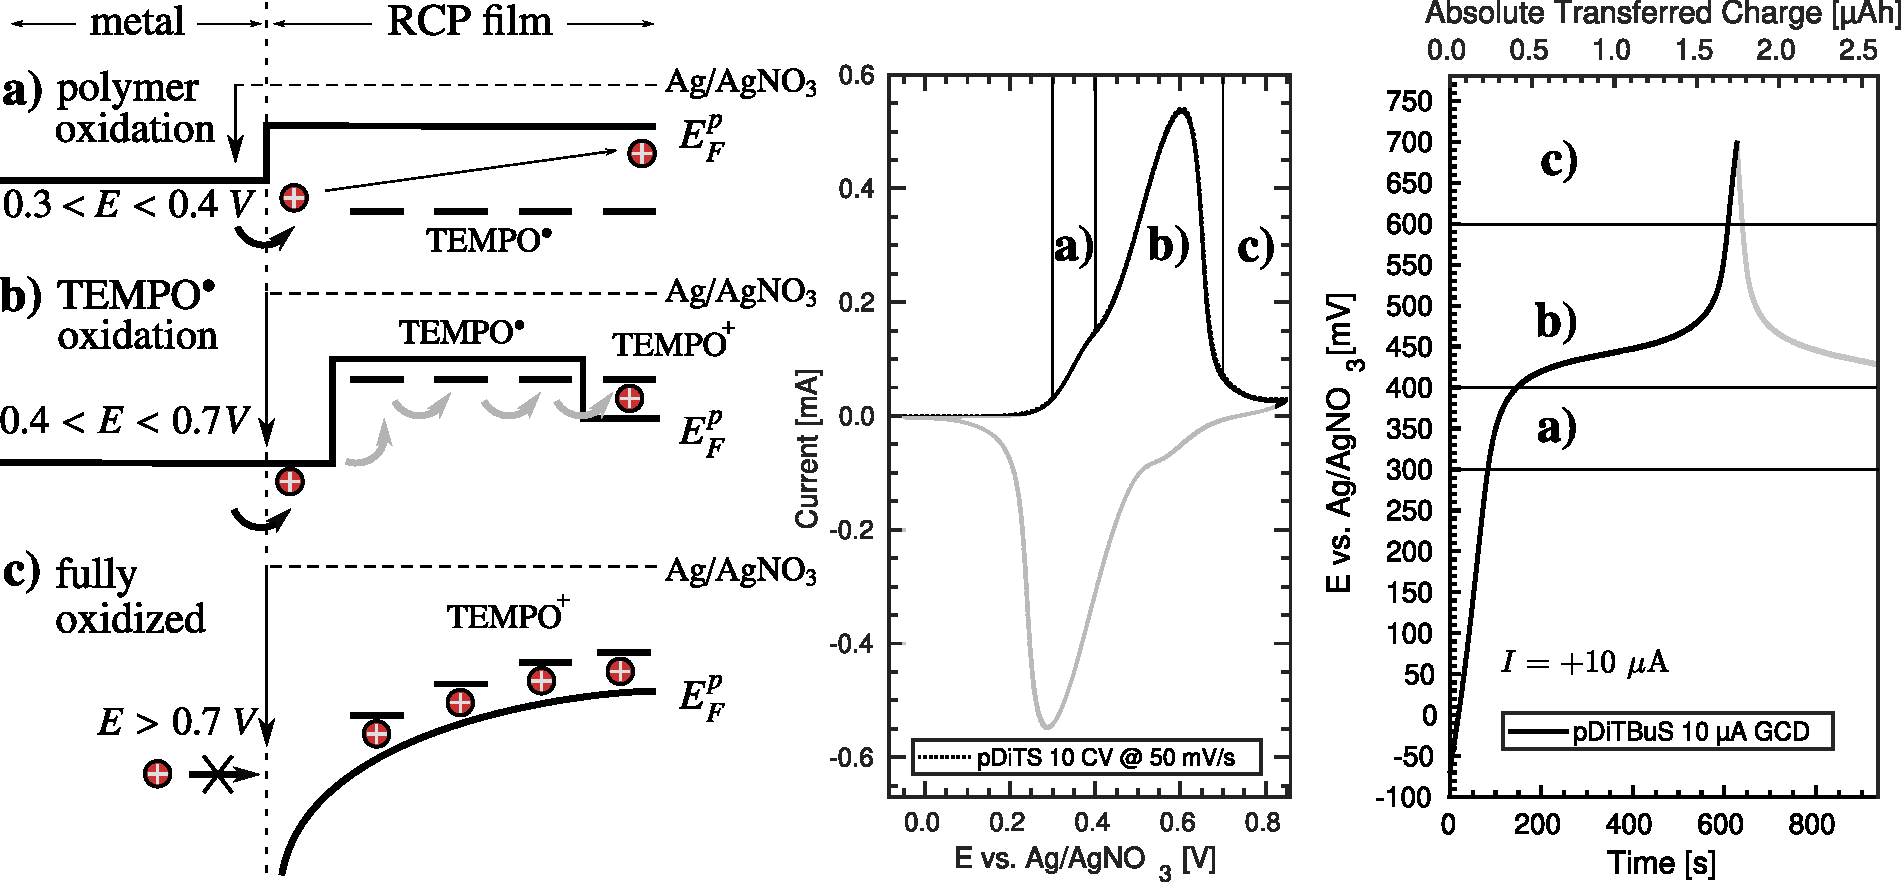
\includegraphics[width=1\textwidth]{./electrochemistry/figures/transport_in_film.pdf}
	\caption{Charging of a poly-TEMPO-Salen film by injecting positive charge carriers at different biasing conditions. The Fermi energy for holes in the film is lowering during its electrochemical p-doping. a) $0.3<E<0.4$~V - the biasing potential is above the oxidation potential of the backbone and below the oxidation potential of TEMPO$^{\bullet}$. b): $0.4<E<0.7$~V - the biasing potential is in the range of the oxidation potentials of TEMPO observed as a current peak in a cyclic voltammogram (middle plot) and a voltage plateau in a galvanostatic charging curve (right plot). c): $E>0.6...0.7$~V - the biasing potential is above the oxidation potential of all TEMPO groups in the film. Bending of the conduction band edge at the metal-semiconductor interface due to the Coulomb shielding by the ions stabilizing the TEMPO$^+$ fragments.}
	\label{fig:biasing_charging}
\end{figure}


